\chapter{Návrh systému}
\label{kap_navrh_systemu}
V předchozích dvou kapitolách byla rozebrána teoretická část problému. V této kapitole shrneme požadavky vyplývající z teorie, které je nutno zakomponovat do
výsledného systému. Nejprve bude schématicky vyjádřena obecná funkcionalita systému, která se následně bude rozebírat detailněji.

\section{Teoretické požadavky}
Nároky na systém, které vyplývají z teorie můžeme rozdělit do třech částí - implementace SNMP protokolu, implementace navrženého XML protokolu a propojení těchto dvou protokolů dohromady.

Hlavním požadavkem, který vyplývá i ze zadání práce, je vytvořit modulární systém, který bude nejenom spojovat současné verze protokolů, ale bude počítat i s potenciálním rozšířením do
budoucna. Obecné schéma navrhovaného systému zobrazuje obrázek \ref{obr_an_obecne_schema}. 

\begin{figure}[htp]
	\begin{center}
		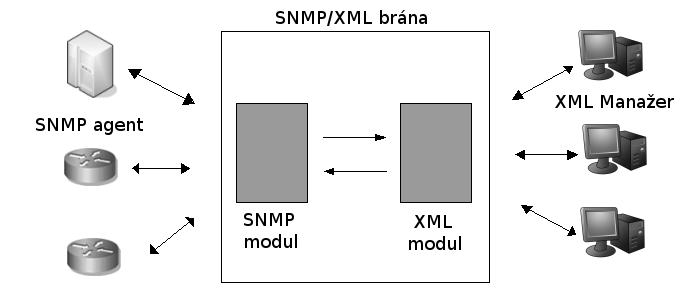
\includegraphics[width=15cm]{obrazky/04_obecne_schema.png}
		\caption{Schéma navrhovahého systému}
		\label{obr_an_obecne_schema}
	\end{center}
\end{figure}

Zde je vidět, že oba dva protokolové moduly jsou na sobě nezávislé a jejich interakce spočívá v předávání si zpráv. Nyní přejděme k detailnějším požadavkům na výše zmíněné části systému.

V rámci \textit{SNMP protokolu} je požadováno
\begin{itemize}
	\item implementace komunikačních struktur protokolů SNMPv1 a SNMPv2
	\item převzetí bezpečnostního schématu z tohoto protokolu
\end{itemize}

\textit{XML orientovaná část programu } má za úkol
\begin{itemize}
	\item implementovat komunikační struktury navrženého protokolu
	\item navrhnout efektivní správu XML struktur v paměti
	\item poskytnout XML manažerům transparentní získání dat z monitorovaných zařízení
	\item mapovat rozšířenou množinu funkcí v rámci XML protokolu do SNMP
	\item s manažery komunikovat pouze přes HTTP/HTTPS protokol
\end{itemize}
Spojením protokolů je myšlen přechod od databázových struktur jednoho protokolu k druhému. V našem případě je to transformace SNMP MIB do XML, jak bylo vysvětleno v kapitole \ref{kap_xml}.

\subsection{XML}
Nejprve se zaměříme na reprezentaci dat, které budou v rámci XML popisovat jak bránu, tak monitorované zařízení. Z předchozích kapitol vyplynulo, že bude použito částečně objektového přístupu a přímého mapování MIB.
Strukturu dat bude popisovat XML dokument, strom, který má strukturu vyjádřenou na obrázku \ref{obr_an_strom_struktura}.

\begin{figure}[htp]
	\begin{center}
		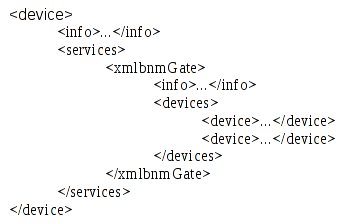
\includegraphics{obrazky/04_schema_dokumentu.png}
		\caption{Obecná struktura XML dokumentu}
		\label{obr_an_strom_struktura}
	\end{center}
\end{figure}

Kořenový uzel specifikuje celé zařízení vystupující jako protokolová brána, obsahuje tyto elementy:
\begin{itemize}
	\item \textbf{info} - tento element obsahuje text, kterým je popsáno dané zařízení.
	\item \textbf{services} - element vymezující poskytované služby (při širší implementaci může obsahovat služby DNS, DHCP, apod.)
	\item \textbf{xmlbnmGate} - naše služba poskytující spojení XML a SNMP protokolu
	\item \textbf{device} - je podelementem \textbf{xmlbnmGate} a vymezuje jedno monitorované zařízení
\end{itemize}

Prvky \textbf{device} jsou do XML dokumentu přidávány na základě informací v konfiguračním souboru (viz kapitola \ref{sec_an_struktura_programu}).

Strukturu elementu \textbf{device} popisuje obrázek \ref{obr_an_device_struktura}. Každý takovýto element bude obsahovat následující informace:
\begin{itemize}
	\item \textbf{info} - stejně jako kořenový element popisuje dané zařízení
	\item \textbf{notifications} - obsahuje elementy a typy upozornění (TRAP zprávy v rámci SNMP), na které manažer čeká
	\item \textbf{subscriptions} - obsahuje informace o datech, které si nechává manažer posílat v pravidelných intervalech (více v popisu komunikace)
	\item \textbf{data} - sem jsou mapována veškerá data přímo z MIB.
\end{itemize}

Samotný element má atribut \textit{id}, což je jeho identifikace v rámci xml dokumentu. Dle tohoto unikátního čísla je pak možné
v sadě dotazů rozpoznat, ke kterému zařízení se dotaz vztahuje.

%\begin{figure}[htp]
%	\begin{center}
%		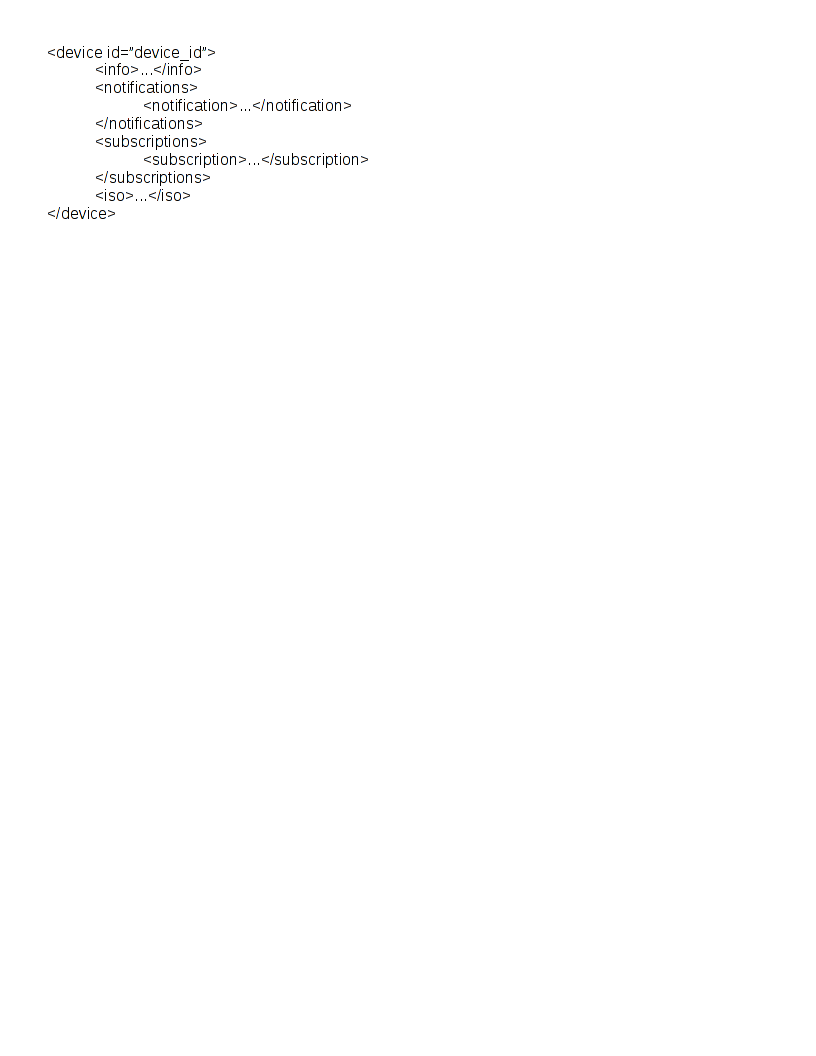
\includegraphics{obrazky/04_schema_device.png}
%		\caption{Struktura elementu device}
%		\label{obr_an_device_struktura}
%	\end{center}
%\end{figure}

Element \textbf{info} obsahuje elementy, které specifikují jméno a popis zařízení (viz obrázek \ref{obr_an_info_element}).

%TODO: doplnit obrazek
%\begin{figure}[htp]
%	\begin{center}
%		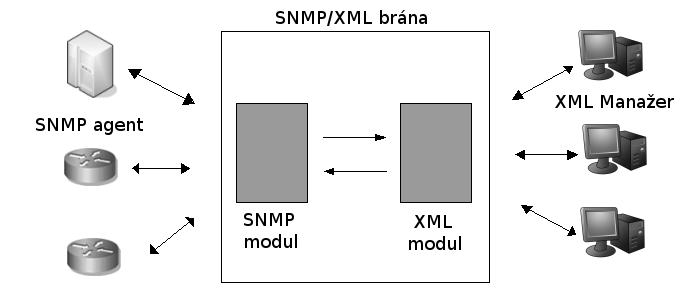
\includegraphics[width=15cm]{obrazky/03_obecne_schema.png}
%		\caption{Schéma navrhovahého systému}
%		\label{obr_an_obecne_schema}
%	\end{center}
%\end{figure}

Jednotlivé podelementy uzlu \textbf{subscriptions} musí z podstaty věci obsahovat informace, které určují, jaké objekty chce manažer pravidelně sledovat, identifikovat
manažera, aby mu mohly být data doručena a specifikovat časový interval, tj. frekvenci sledování příslušné veličiny.

Děti uzlu \textbf{notifications} určují, které typy událostí jsou sledovány u daného zařízení. V rámci konfigurace systému je nezbytné, aby pro každé zařízení
bylo jasně definováno, kam mají být příslušné zprávy o událostech zasílány. Tudíž v rámci typu události je nutné uvést příjemce, který bude zprávy očekávat. Přesná 
specifikace jednotlivých uzlů dokumentu je v příloze 
%TODO dopsat referenci na prilohu, kde jsou specifikace jednotlivych uzlu

Mapování dat z MIB bylo obecně popsáno v kapitole \ref{kap_xml} a přesný algoritmus bude specifikován v následující kapitole. Pro adresaci jednotlivých objektů
je, jak bylo již nastíněno v předchozí kapitole, použito mechanismů XPath či XQuery. Dotaz na položku z MIB může vypadat následovně
\begin{verbatim}
	/device/services/xmlbnmgate/device[id=1]/data/...
\end{verbatim}

\subsubsection*{Zprávy}
Zprávy, které budou posílány mezi manažerem a bránou, mají formu XML dokumentu. Schématicky je znázorněna a popsána v kapitole \ref{kap_xml}, obrázek .
%TODO dodat cislo obrazku odkazujici na message format v ramci xml kapitoly

Kořenový element message obaluje veškerá posílaná data. Může obsahovat několik dílčích dotazů, nastavení a ostatních informací, které budou vykonávány postupně
jedna po druhé. V rámci teorie byla nastíněna možnost použití několika různých front, které by byly specifikovány identifikátorem a zaručovaly by různou
prioritu zpracování. Navrhovaný systém bude podporovat pouze jednu frontu zpracování zpráv, čímž budou jednotlivé dotazy zpracovány postupně. Bude tak zaručena
integrita dat a předejde se různým extrémním situacím.

Komunikace mezi manažerem a bránou je na XML úrovni omezena na zprávy
\begin{itemize}
	\item GET
	\item SET
	\item DISCOVERY
	\item PUBLICATION
	\item SUBSCRIPTION
	\item DISTRIBUTION
	\item EVENT
\end{itemize}

Přesná struktura a popis funkce jednotlivých zpráv byla popsána v předchozí kapitole.


\subsubsection*{Komunikační protokol}
Od protokolu SNMP se XML část komunikace liší taky tím, že bude probíhat na spolehlivém a potvrzovaném protokolu - HTTP. Každá zpráva, která
je poslána, musí mít potvrzeno doručení, což tento aplikační protokol, využívající transportního protokolu TCP, nabízí. 

Informace budou posílány ve formátu HTTP POST zprávy. Strukturu dotazu a odpovědi zobrazuje obrázek \ref{obr_an_post_zprava}.

%TODO: doplnit obrazek
%\begin{figure}[htp]
%	\begin{center}
%		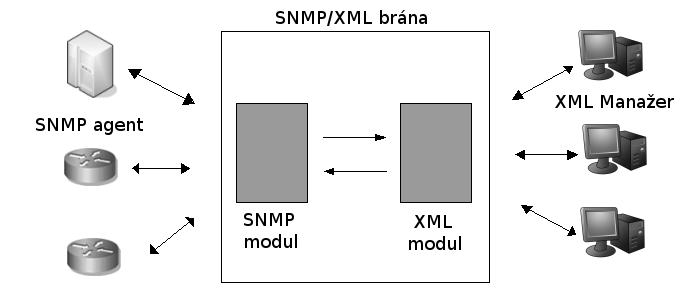
\includegraphics[width=15cm]{obrazky/03_obecne_schema.png}
%		\caption{Schéma navrhovahého systému}
%		\label{obr_an_obecne_schema}
%	\end{center}
%\end{figure}

Otázka bezpečného přenosu dat byla řešena v předchozí kapitole a byl zvolen protokol HTTPS. Zajištění distribuce a zpracování certifikátů bude
diskutováno dále v této kapitole.


\subsection{SNMP}
Druhou část komunikace tvoří SNMP protokol. Z kapitoly \ref{kap_analyza} vychází seznam zpráv, které je nutné implementovat:
\begin{itemize}
	\item Get
	\item Set
	\item Response
	\item GetNext
	\item Trap
\end{itemize}

V rámci komunikace se v naší práci budeme zaobírat verzemi SNMPv1 a SNMPv2. Samotná implementace a mapování SNMP zpráv na XML dotazy
bude diskutována až v kapitole \ref{kap_implementace}.

Bezpečnost se v SNMP omezuje pouze na komunitní heslo, které je zasíláno jako součást XML zprávy a bude pouze přepsáno do SNMP paketu. 
Je tedy zřejmé, že ponecháváme bezpečnost takovou, jak je standardizována v SNMP protokolu.


\section{Struktura programu}
\label{sec_an_struktura_programu}
%TODO
%krok za krokem vyjadrit, jak bude program nabihat a bezet
%config file navrhnout
%build XML tree  (transform from MIB)
%atd atd (viz struktura_programu v analyze)
%DISKUSE embedded http server/ outsource http server
%DISKUSE na SOAP vs. demon
%DISKUSE ohledne sdileni nodu v xml stromu

\section{Manager}
%TODO: zahrnout nutnost udelani i manazera
